% Mirror: https://github.com/SIGma-UIUC/presentation-format
% --------------------------------------------------------------------
% This is a simple Beamer document that uses beamerthemesigma.sty
% Reading the comments should help you create a presentation even if
% you've never used Beamer before.
% --------------------------------------------------------------------

\documentclass[aspectratio=169]{beamer}
% \documentclass[aspectratio=169, handout]{beamer}
% Add handout option to ignore pauses

% From Jeff E
\usepackage{algo}
\usepackage{sigmastyle}
\usepackage{mathdots}

\setbeamertemplate{blocks}[rounded]
\setbeamercovered{transparent}
\usecolortheme{orchid}
\usetheme{sigma}

\title{Inverse Ackermann Function}
\author{Ian Chen}
\date{}

% \institute{University of Illinois Urbana-Champaign}

% --------------------------------------------------------------------

% Begin document
\begin{document}

\begin{frame}
	\titlepage
\end{frame}

\begin{frame}{Outline}
	\tableofcontents
\end{frame}

\section{The Function}
\frame{\sectionpage}

\begin{frame}{Motivation}
	This function is meant to capture different orders of growth.
	\pause
	\begin{enumerate}
		\item linear \pause
		\item logarithmic \pause
		\item iterated logarithmic
	\end{enumerate}
\end{frame}

\begin{frame}{Tarjan's Definition}
	\begin{defn}[Tarjan '75]
		\[
			A(i, j) =
			\begin{cases}
				2j                    & \for \ i = 0 \land j \ge 1 \\
				1                     & \for \ i \ge 1 \land j = 0 \\
				A(i - 1, A(i, j - 1)) & \ow
			\end{cases}
		\]
	\end{defn}
	\pause
	\begin{defn}[Tarjan '75]
		\[
			\alpha(i, x) = \min \set{j | A(i, j) \ge x}
		\]
	\end{defn}
\end{frame}

\begin{frame}{Definition}
	\begin{defn}
		\[
			\alpha(i, j) =
			\begin{cases}
				0                               & \for \ j = 1             \\
				\floor{j / 2}                   & \for \ i = 1 \land j > 1 \\
				\pause
				1 + \alpha(i, \alpha(i - 1, j)) & \ow
			\end{cases}
		\]
	\end{defn}
	\pause
	\begin{defn}
		\[
			\beta(i, j) =
			\begin{cases}
				0                             & \for \ j = 1             \\
				\floor{\sqrt{j}}              & \for \ i = 1 \land j > 1 \\
				\pause
				1 + \beta(i, \beta(i - 1, j)) & \ow
			\end{cases}
		\]
	\end{defn}
\end{frame}

\begin{frame}{A sequence of functions}
	\pause
	\begin{minipage}{0.48\linewidth}
		\onslide<+->
		\begin{itemize}
			\item $ \alpha(1, n) = \floor{n / 2} $
			      \onslide<+->
			\item $ \alpha(2, n) = \lg n $
			      \onslide<+->
			\item $ \alpha(3, n) = \lg^* n $
		\end{itemize}
	\end{minipage}
	\begin{minipage}{0.48\linewidth}
		\onslide<+->
		\begin{itemize}
			\item $ \beta(1, n) = \floor{\sqrt n} $
			      \onslide<+->
			\item $ \beta(2, n) = \lg \lg n $
		\end{itemize}
	\end{minipage}
\end{frame}

\section{RMQ Preprocessing}
\frame{\sectionpage}

\begin{frame}{A Short but Cute Result}
	Suppose we are given an array of $n$ integers.
	We want to be able to answer \emph{range minimum queries} in few steps.

	\pause
	\begin{eqn}
		$$
			\lambda(2k, n) = \alpha(k, n) \qquad
			\lambda(2k + 1, n) = \beta(k, n)
		$$
	\end{eqn}
	\pause
	\begin{thrm}[Alon '87]
		We can answer range minimum queries in $k$ steps using $\mathcal{O}(nk \lambda(k, n))$ preprocessing space.
	\end{thrm}

\end{frame}

\begin{frame}{Divide and Conquer}
	Let $T_k(n)$ be the time to preprocess an array of $n$ elements for $k$-step queries.
	\pause
	\begin{eqn}
		$$
			T_2(n) = 2n \lg n
		$$
		$$
			T_3(n) = 3n \lg \lg n
		$$
		$$
			T_k(n) = \dfrac{n}{\lambda(k - 2, n)} T_k(\lambda(k - 2, n)) + T_{k-2}(n / \lambda(k - 2, n)) + 2n
		$$
	\end{eqn}
	\pause
	\begin{eqn}
		$$
			T_k(n) = \mathcal{O}(nk \lambda(k, n))
		$$
	\end{eqn}
\end{frame}

\begin{frame}{Additional Results}
	\begin{itemize}\onslide<+->
		\item The analysis is tight. \onslide<+->
		\item The best linear time preprocessing takes $\alpha(n)$  steps. \onslide<+->
		\item Tree queries, linear queries.
	\end{itemize}
\end{frame}

\section{Disjoint Sets}

\frame{\sectionpage}

\begin{frame}{Union-Find}
	Given a set of elements, label them $1$ through $n$.
	We want to partition these elements into buckets, supporting
	the operations
	\begin{itemize} \onslide<+->
		\item \textsc{Union} \onslide<+->
		\item \textsc{Find}
	\end{itemize}
\end{frame}

\begin{frame}{Implementation}
	\begin{minipage}{0.48\textwidth}
		\onslide<+->
		\begin{algo}
			\textul{\textsc{Find}($x$)}: \+
			\\ $y \gets x$
			\\ while $y \ne \emph{parent}(y)$ \+
			\\ $y \gets \emph{parent}(y)$ \-
			\\ $\textsc{Compress}(x, y)$
			\\ return $x$
		\end{algo}
	\end{minipage}
	\begin{minipage}{0.48\textwidth}
		\onslide<+->
		\begin{algo}
			\textul{\textsc{Compress}($x$, $y$)}: \+
			\\ if $x \ne y$ \+
			\\ $\textsc{Compress}(\emph{parent}(x), y)$
			\\ $\emph{parent}(x) \gets \emph{parent}(y)$
		\end{algo}
	\end{minipage}
\end{frame}

\begin{frame}{Implementation}
	\begin{minipage}{0.6\textwidth}
		\onslide<+->
		\begin{algo}
			\textul{\textsc{UnionLeader}($x$, $y$)}: \+
			\\ if $ \emph{rank}(x) > \emph{rank}(y) $ \+
			\\ $\emph{leader}(y) \gets x$ \-
			\\ else \+
			\\ $\emph{leader}(x) \gets y$
			\\ if $ \emph{rank}(x) = \emph{rank}(y) $ \+
			\\ $\emph{rank}(x) \gets \emph{rank}(x) + 1$
		\end{algo}
	\end{minipage}
	\begin{minipage}{0.38\textwidth}
		\onslide<+->
		\begin{algo}
			\textul{\textsc{Union}($x$, $y$)}: \+
			\\ $\overline{x} \gets \textsc{find}(x)$
			\\ $\overline{y} \gets \textsc{find}(y)$
			\\ \textsc{UnionLeader}($\overline{x}$, $\overline{y}$)
		\end{algo}
	\end{minipage}
\end{frame}

\begin{frame}{Analysis}
	\begin{enumerate}  \onslide<+->
		\item leader ranks only increase \onslide<+->
		\item \emph{parent}$(x)$ has lower rank than $x$ \onslide<+->
		\item \emph{size}$(\overline{x})$ is at least $2^{\emph{rank}(\overline{x})}$\onslide<+->
		\item For any rank $r$, there are at most $n/2^r$ elements of rank $r$
	\end{enumerate}
\end{frame}

\begin{frame}{Analysis}
	\begin{enumerate}\onslide<+->
		\item Amortized analysis \onslide<+->
		\item Number of pointer operations \onslide<+->
		\item \textsc{Find} is dominated by \textsc{Compress}\onslide<+->
		\item can make all calls to \textsc{UnionLeader} before \textsc{Compress}\onslide<+->
		\item can \textsc{Shatter} the tree into two forests
	\end{enumerate}
\end{frame}

\begin{frame}{Compress and Shatter}
	\begin{algo}
		\textul{\textsc{Compress}($x$, $y$, $F$)}: \+
		\\ if $\emph{rank}(x) \ge s$ \+
		\\ \textsc{Compress}($x$, $y$, $F_+$) \-
		\\ else if $\emph{rank}(y) < s$ \+
		\\ \textsc{Compress}($x$, $y$, $F_-$) \-
		\\ else \+
		\\ $z \gets x$
		\\ while $\emph{rank}(z) < s$ \+
		\\ $z' \gets \emph{parent}(z)$
		\\ $\emph{parent}(z) \gets z$
		\\ $z \gets z'$ \-
		\\ $\emph{parent}(z) \gets z$
		\\ \textsc{Compress}($\emph{parent}(z), y, F_+$)
	\end{algo}
\end{frame}

\begin{frame}{Analysis}
	\begin{center}
		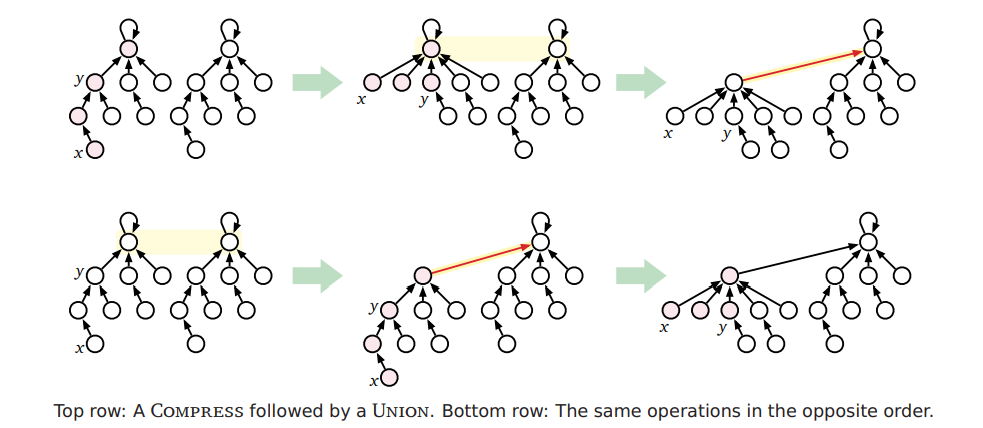
\includegraphics[width=\textwidth]{union_compress_reorder.png}
	\end{center}
\end{frame}

\begin{frame}{Analysis}
	\begin{center}
		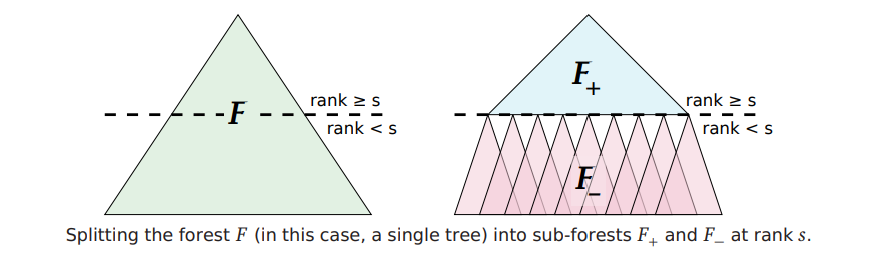
\includegraphics[width=\textwidth]{partition_forest.png}
	\end{center}
\end{frame}

\begin{frame}{Analysis}
	\begin{center}
		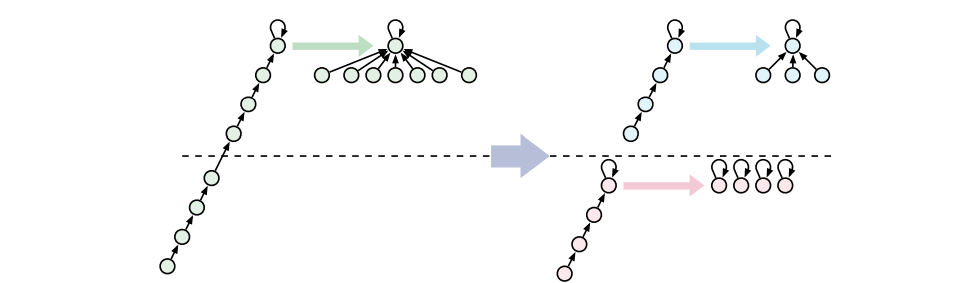
\includegraphics[width=\textwidth]{shatter.png}
	\end{center}
\end{frame}

\begin{frame}{Analysis}
	Let $T(m, n, r)$ be the number of pointer operations
	that $m$ \textsc{Compress} operation takes, on a tree
	with $n$ nodes and maximum rank $r$.

	\pause
	\begin{thrm}
		$$
			T(m, n, r) \le nr
		$$
	\end{thrm}
\end{frame}

\begin{frame}{Analysis}
	Consider the sequences of $m_+$ and $m_-$
	\textsc{Compress} calls on $F_+$ and $F_-$.

	\pause
	\begin{eqn}
		$$
			T(m, n, r) \le T(m_+, n_+, r) + T(m_-, n_-, r) + m_+ + n
		$$
	\end{eqn}
\end{frame}

\begin{frame}{Analysis}
	Let $s = \lg r$.

	\pause
	Since $n_+ < n/2^s$, we have that
	\begin{eqn}
		$$
			T(m_+, n_+, r) \le rn_+ \le rn/2^s = n
		$$
		$$
			T(m, n, r) \le T(m_-, n_-, \lg r) + m_+ + 2n
		$$
	\end{eqn}

	\pause
	Letting $T'(m, n, r) = T(m, n, r) - m$,
	\begin{eqn}
		$$
			T'(m, n, r) \le T'(m, n, \lg r) + 2n
		$$
	\end{eqn}

	\pause
	\begin{thrm}
		$$
			T(m, n, r) \le m + 2n \lg^* r
		$$
	\end{thrm}
\end{frame}

\begin{frame}{Analysis}
	Let $s = \lg^* r$.

	\pause
	Since $n_+ < n/2^s$, we have that
	\begin{eqn}
		$$
			T(m_+, n_+, r) \le m_+ + 2n_+ \lg^* r \le m_+ + 2n \dfrac{\lg^* r}{2^{\lg^* r}} \le m + 2n
		$$
	\end{eqn}

	\pause
	Letting $T'(m, n, r) = T(m, n, r) - 2m$,
	\begin{eqn}
		$$
			T'(m, n, r) \le T'(m, n, \lg^* r) + 3n
		$$
	\end{eqn}

	\pause
	\begin{thrm}
		$$
			T(m, n, r) \le 2m + 3n \lg^{**} r
		$$
	\end{thrm}
\end{frame}

\begin{frame}{Analysis}
	\begin{thrm}
		$$
			T(m, n, r) \le cm + (c+1)n \lg^{*^{c}} r
		$$
	\end{thrm}

	\pause

	\begin{eqn}
		$$
			T(m, n, r) \le cm + (c+1)n \alpha(c, r)
		$$
	\end{eqn}

	\pause

	\begin{thrm}
		$$
			T(m, n, r) \le m \alpha(n)
		$$
	\end{thrm}
\end{frame}

\begin{frame}{}
	\begin{center}
		{\color{sigma@mainblue} \LARGE Questions?}
	\end{center}
\end{frame}

\begin{frame}{Brainteaser (Erickson)}
	Consider the following game. I choose a positive integer n and keep it secret; your goal is
	to discover this integer. We play the game in rounds. In each round, you write a list of at
	most n integers on the blackboard. If you write more than n numbers in a single round,
	you lose. If n is one of the numbers you wrote, you win the game; otherwise, I announce which of
	the numbers you wrote is smaller or larger than n, and we proceed to the next round.

	Describe a strategy that wins in $\mathcal{O}(\alpha(n))$ rounds.
\end{frame}

\font\eightss=cmssq8
\font\eightssi=cmssqi8
\newcommand\quoteAuthorDate[3]{\begingroup
	\baselineskip 10pt
	\parfillskip 0pt
	\interlinepenalty 10000 % not needed in example
	\leftskip 0pt plus 40pc minus \parindent
	\let\rm=\eightss
	\let\sl=\eightssi
	\everypar{\sl}#1\par
	\nobreak\smallskip
	\noindent\rm--- #2\unskip\enspace(#3)\par
	\endgroup}
\begin{frame}
	\begin{center}
		\item \quoteAuthorDate{WAGA WAGA}{Sariel Har-Peled}{\textcolor{sigma@mainblue}{2024}}
		\item \quoteAuthorDate{All problems in computer science can be solved by another level of indirection.}{David Wheeler}{\textcolor{sigma@mainblue}{2014}}
	\end{center}
\end{frame}

\begin{frame}[allowframebreaks]{Bibliography}
	\bibliography{refs}
	\bibliographystyle{alpha}
	\begin{itemize}
		\item Tar75, Tarjan, \textit{Efficiency of a good but not linear set union algorithm}
		\item Alon87, Alon \& Schieber, \textit{Optimal Preprocessing for Answering On-Line Product Queries}
		\item Jeffe, Erickson, \textit{Data Structures for Disjoint Sets}
	\end{itemize}
\end{frame}

\end{document}
